\chapter{Fig, table and Code}

\section{Figure}

\begin{figure}[htb]
  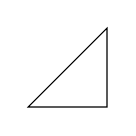
\begin{tikzpicture}
    \draw (0,0) -- (1, 0) -- (1, 1) -- cycle;
  \end{tikzpicture}
  \caption{An example tikz picture with long caption: \blindtext\\\blindtext}
  \label{fig:tikz example}
\end{figure}

You can use \lstinline|\cref{}| to automatically setup the cross reference name; instead, you can always use \lstinline|\ref{}| to customize the appearence of the cross reference.

An example image is shown in \cref{fig:tikz example} or Figure (\ref{fig:tikz example}).

\section{Code}

\subsection{Inline code}
Use \lstinline$\lstinline|<code>|$ to print code snippets. The \lstinline$||$ marks delimit
the code and can be replaced by any character not in the code;
\textit{e.g.}   \lstinline|\lstinline$<code>$| gives the same result.

\subsection{Code environment}
The code to draw the \cref{fig:tikz example} is listed below:
\begin{lstlisting}[caption={\hologo{LaTeX} code for inserting a figure}]
\begin{figure}[htb]
  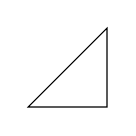
\begin{tikzpicture}
    \draw (0,0) -- (1, 0) -- (1, 1) -- cycle;
  \end{tikzpicture}
  \caption{An example picture with long caption: \blindtext\\\blindtext}
  \label{fig:tikz example} % this is a comment
\end{figure}
\end{lstlisting}

\subsection{Enumitem}

\begin{itemize}
  \item Test test.
  \item Test test.
  \item Test test.
  \begin{itemize}
    \item test test
    \item test test\footnote{\blindtext}
    \item test test
    \item test test
  \end{itemize}
  \item Test test.
\end{itemize}

\begin{enumerate}
  \item Test test.
  \item Test test.
  \item Test test.
  \begin{enumerate}
    \item test test
    \item test test\footnote{\blindtext}
    \item test test
    \item test test
  \end{enumerate}
  \item Test test.
\end{enumerate}

